\begin{enumerate}
	\item Exercício retirado da página 1023 de \cite{James_Stewart_calculo_v2}
	
	Calcule $$\iiint_E x^2\, dv$$, onde $E$ é o solido que está dentro do cilindro $x^2 + y^2 = 1$, acima do plano $z = 0$ e abaixo do cone $z^2 = 4x^2 + 4y^2$.
	
	\begin{figure}[htb]
		\caption{Coordenadas cilíndricas - Aula 08 - Exercício I}
		\label{v32_a08_e01}
		\centering
		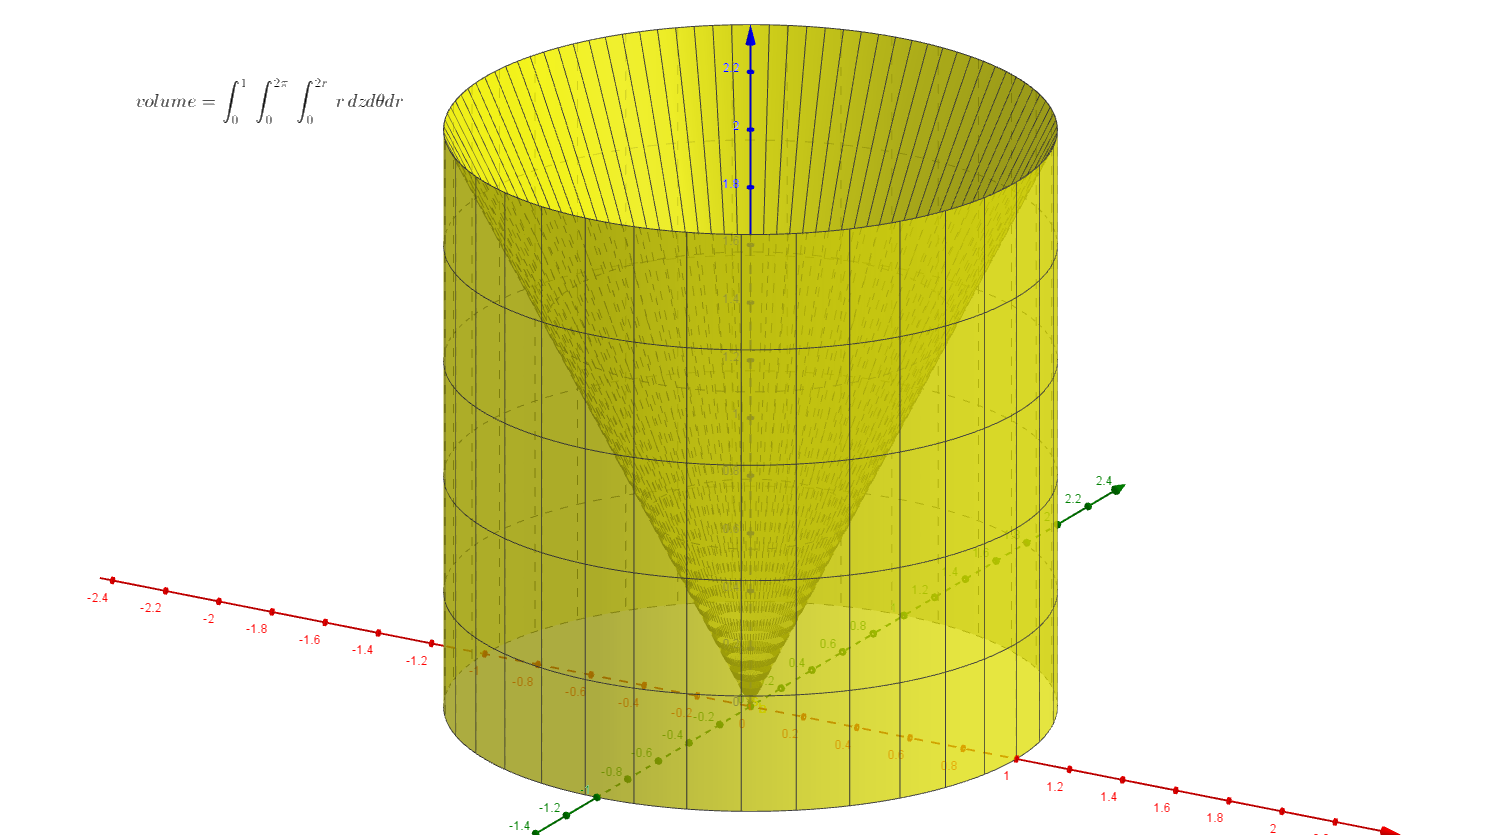
\includegraphics[width=0.5\textwidth]{v32_a08_e01.png}		
	\end{figure}
	
	\begin{equation*}
		x^2 + y^2 = 1 \Rightarrow r^2 = 1 \Rightarrow r = 1
	\end{equation*}
	\begin{equation*}
		z^2 = 4x^2 + 4y^2 = 4\left(x^2 + y^2\right) = 4r^2 \Rightarrow z = \pm\sqrt{4r^2} = \pm 2r 
	\end{equation*}
	\begin{equation*}
		0 \leq r \leq 1,\, 0 \leq \theta \leq 2\pi,\, 0 \leq z \leq 2r
	\end{equation*}
	\begin{equation*}
		x^2 = \left(r\cos(\theta)\right)^2 = r^2\cos^2(\theta)
	\end{equation*}
	\begin{gather*}
		\int_0^1 \int_0^{2\pi} \int_0^{2r} \left(r^2\cos^2(\theta)\right)r\,dz d\theta dr = \int_0^1 r^3\, dr \int_0^{2\pi} \cos^2(\theta)\, d\theta \int_0^{2r} dz =\\ \int_0^1 r^3\, dr \int_0^{2\pi} \cos^2(\theta)\, d\theta \left[z\right]_0^{2r} = 2\int_0^1 r^4\, dr \int_0^{2\pi} \cos^2(\theta)\, d\theta =\\ {\overstrike{2}}\int_0^1 r^4\, dr \int_0^{2\pi} \dfrac{1 + \cos(2\theta)}{\overstrike{2}}\, d\theta = \left[\dfrac{r^5}{5}\right]_0^1 \int_0^{2\pi} \left(1 + \cos(2\theta)\right) d\theta =\\ \dfrac{1}{5} \left(\int_0^{2\pi} d\theta + \int_0^{2\pi}\cos(u) \dfrac{du}{2}\right) = \dfrac{1}{5} \left(\int_0^{2\pi} d\theta + \dfrac{1}{2}\int_0^{2\pi}\cos(u)\,du\right)	=\\ \dfrac{1}{5} \left[\theta + \dfrac{\sen(u)}{2}\right]_0^{2\pi}	= \dfrac{1}{5} \left[\theta + \dfrac{\sen(2\theta)}{2}\right]_0^{2\pi} = \dfrac{1}{5} \left[\theta + \dfrac{\overstrike{2}\sen(\theta)\cos(\theta)}{\overstrike{2}}\right]_0^{2\pi} =\\ \dfrac{1}{5} \left[2\pi \overstrike{+ \sen(2\pi)\cos(2\pi)} \overstrike{- \left(0 + \sen(0)\cos(0)\right)}\right] = \frac{2\pi}{5}
	\end{gather*}
	\begin{equation*}
		u = 2\theta \Rightarrow \dfrac{du}{2} = d\theta        
	\end{equation*}
\end{enumerate}